\documentclass[10pt]{article}
\usepackage[a4paper,margin=15mm]{geometry}
\usepackage[no-math]{fontspec}
\setmainfont{Latin Modern Roman}
\usepackage{amsmath,amsfonts,amssymb,amsthm,graphicx,xurl,enumitem}
\usepackage[unicode,hidelinks]{hyperref}
\newtheorem{theorem}{Theorem}[section]
\newtheorem{lemma}[theorem]{Lemma}
\newtheorem{remark}[theorem]{Remark}
\newtheorem{definition}[theorem]{Definition}
\newtheorem{proposition}[theorem]{Proposition}
\newtheorem{conjecture}[theorem]{Conjecture}
\newtheorem{question}{Question}
\allowdisplaybreaks
\setlength\emergencystretch{3em}
% Exact finite authored ordinary-notation definitions, with source line pins below.
\newcommand{\cL}{\mathcal{L}}
\newcommand{\cU}{\mathcal{U}}
\newcommand{\cV}{\mathcal{V}}
\newcommand{\cW}{\mathcal{W}}
\newcommand{\bF}{\mathbf{F}}
\newcommand{\N}{\mathbb N}
\newcommand{\F}{\mathbb F}
\newcommand{\e}{\varepsilon}
\newcommand{\Fp}{\mathbb{F}_p}
\newcommand{\R}{\mathbb{R}}
\newcommand{\si}{\sigma}
\newcommand{\bzz}{\mathbf{0}}
\newcommand{\lam}{\lambda}
\begin{document}\begin{center}\Large Problem2476: Prime-field Furstenberg upper construction\end{center}\noindent\textbf{Author:} Shengwen Gan\par\noindent\textbf{Work/version:} Exceptional set estimate in prime fields: dimension two implies higher dimensions; Exact arXiv 2409.11637v2, 28 September 2025, native CC BY 4.0; byte-matching published Discrete Analysis 2025:19, 55 pp., 29 September 2025, DOI 10.19086/da.144860, PDF CC BY 3.0\par\noindent\textbf{Native source/license:} \url{https://arxiv.org/src/2409.11637v2}; \url{https://creativecommons.org/licenses/by/4.0/}\par\noindent\textbf{Published companion:} CC BY3.0, \url{http://creativecommons.org/licenses/by/3.0/}\par\noindent\textbf{Difficulty:} H1: The all-parameter construction coordinates planar incidences, dimension lifting and transverse affine-plane multiplicities to attain the piecewise Furstenberg exponent. The authored product construction handles fractional incidence exponents and the saturated final regime without the conjectural lower bound. Every required planar and higher-dimensional construction is retained.\par\medskip\noindent\textbf{Editorial source boundary:} Theorem1.7 is the sole selected unconditional upper construction for every admissible n,k,s,t and prime p. Full Furstenberg-set/admissibility/asymptotic notation and every piecewise index definition are retained. The complete planar rectangle/slope construction2.3, its original ceil convention, full Grassmann/transversality lemma2.7 and the entire unwrapped Section3 upper proof through all cases(a)-(d) are included. Euclidean Ren-Wang background and the planar conjecture remain source context; the selected result does not assume that conjecture. The conditional lower result1.8/2477 and projection results are unselected and uncounted. The original Section3.2 introductory target at986 uses the opposite lower-bound sign while the selected statement and actual constructions print upper bounds; both forms remain unchanged. The literal tau> wording at1018 and the final nested superscript/braces at1063 also remain exact; no parameter or equality tokens are repaired. OriginalFigure1 is unchanged, and its two printed extent labels have separately marked editable transcriptions. Body excerpts are authentic nativeCC4; these checked published/source-asset labels are a separate component, so canonical mixed origin is conservative checked-published-transcription rather than a claim all mathematical labels were native. Native exactv2 and publishedPDFCC3 grants/versions are distinct. No original publisher class or containing archive is executed/exported.\par\medskip\hrule\medskip\noindent\textbf{Original human-authored mathematics follows.}\par
% Original author source LF lines 322--343

\section{Introduction}

We study the exceptional set estimate and a Furstenberg-type problem in prime fields. The main novelty of this paper is that we prove, for these two problems, that the two-dimensional result implies all higher-dimensional results. 

\subsection{Background}

We first introduce the two problems---the Furstenberg set problem and the exceptional set estimate in Euclidean space.




\subsubsection{Furstenberg set problem}\hfill

The Furstenberg set problem was originally considered by Wolff \cite{wolff1999recent} in $\R^2$. Fix $s\in (0,1], t\in (0,2]$. We say $E\subset \R^2$ is an $(s,t)$-set in $\R^2$, if $E$ is of the form
\[ E=\bigcup_{\ell\in \cL}Y(\ell), \]
where $\cL\subset A(1,\R^2)$ is a set of lines in $\R^2$ with $\dim\cL=t$ and for each $\ell\in \cL$ there exist $Y(\ell)\subset \ell$ with $\dim Y(\ell)=s$. ($\dim$ will always mean Hausdorff dimension.) The Furstenberg set problem asks about the optimal lower bound on the Hausdorff dimension of $(s,t)$-sets, that is,
\[ \inf_{E \textup{~is~a~}(s,t)\textup{-set}}\dim(E). \]
Recently, Ren and Wang \cite{ren2023furstenberg} resolved the Furstenberg set problem by proving
\begin{equation}\label{renwang}
\inf_{E \textup{~is~a~}(s,t)\textup{-set}}\dim(E)=\min\{s+t,\frac{3}{2}s+\frac{1}{2}t,s+1  \}.
\end{equation} 
For more references and history on this problem, we refer to \cite{ren2023furstenberg}, \cite{orponen2023projections}. 
% Original author source LF lines 386--456
\setcounter{theorem}{1}\setcounter{equation}{2}\setcounter{subsection}{1}
\subsection{The problems in prime fields}
In the remainder of the paper, we look only at the prime fields. Let $p$ be a prime and $\Fp$ be the prime field with $p$ elements. Throughout the paper, $A\lessapprox B$ means $A\le  C (\log p)^{C} B$ for some large constant $C$ (independent of $p$). $A\approx B$ means both $A\lessapprox B$ and $B\lessapprox A$.  $A\lesssim B$ means $A\le C B$ for a large constant $C$ (independent of $p$). $A\sim B$ means both $A\lesssim B$ and $B\lesssim A$. 

\subsubsection{Furstenberg set problem}

\begin{definition}[$(s,t;n,k)$-set]
    Fix integers $1\le k<n$, and numbers $0\le s\le k$, $0\le t\le (k+1)(n-k)$. Let $0<\lam\le 1$. We say $E$ is a $(s,t;n,k;\lam)$-Furstenberg set (over $\Fp$), if $E$ is a subset of $\Fp^n$ of form
    \[ E=\bigcup_{V\in\cV}Y(V). \]
    Here, $\cV\subset A(k,\Fp^n)$ is a set of $k$-planes with $\#\cV\ge \lam p^t$; for each $V\in\cV$, $Y(V)$ is a subset of $V$ with $\#Y(V)\ge \lam p^s$. 
\end{definition}

\begin{remark}
   {\rm We remark that $s,t,n,k$ are important parameters, while $\lam$ is not.
   Since $\lambda$ is not an important parameter, from now on we will drop $\lam$ from the notation and simply call $(s,t;n,k;\lam)$-set as $(s,t;n,k)$-set, thinking of $\lam$ as a fixed constant in $(0,1]$. 
   }
\end{remark}

We give the following definition.
\begin{definition}
    We say $(s,t;n,k)$ is admissible if $1\le k<n$ are integers and $0\le s\le k$, $0\le t\le (k+1)(n-k)$.
\end{definition}

The Furstenberg set problem can be formulated as follows:

\begin{question}
Suppose $(s,t;n,k)$ is admissible.
Find the largest $\bF(s,t;n,k)$, so that 
\begin{equation}\label{deff}
    \inf_{E:\ (s,t;n,k)\textup{-set}} \#E\gtrsim_{s,t,n,k,\e} p^{\bF(s,t;n,k)-\e} 
\end{equation}
holds for any $\e>0$.
\end{question}

In the above inequality, the implicit constant may depend on many parameters, but never depends on $p$. For simplicity, we may view $s,t,n,k$ as fixed parameters and write $\gtrsim_{s,t,n,k,\e}$ as $\gtrsim_\e$ throughout the paper. The dependence on $s,t,n,k$ will be mentioned when needed. 
We are interested in the behavior as $p$ goes to infinity, so the goal is to find the index $\bF(s,t;n,k)$ for fixed $(s,t;n,k)$.

We see that the problem consists of two parts:
for fixed $(s,t;n,k)$,
\begin{enumerate}
    \item (Lower bound) show for any $(s,t;n,k)$-set $E$, we have $\#E\gtrsim_{\e} p^{\bF(s,t;n,k)-\e}$;
    \item (Upper bound) show the existence of a $(s,t;n,k)$-set $E$, such that $\#E\lesssim p^{\bF(s,t;n,k)}$.
\end{enumerate}

\medskip

Based on Ren-Wang's result \eqref{renwang}, it is reasonable to make a conjecture in $\Fp^2$.

\begin{conjecture}\label{conj2d}
    Fix $s\in(0,1],t\in (0,2]$. Then for any $(s,t;2,1)$-set $E$ over $\Fp$, we have
    \[ \#E\gtrsim_{s,t,\e} p^{\min\{s+t,\frac{3}{2}s+\frac{1}{2}t,s+1  \}-\e}, \]
    for any $\e>0$.
\end{conjecture}

\begin{remark}
{\rm
    It is crucial to use the prime field $\Fp$. Otherwise, the conjecture fails. Consider the problem in $\F_q^2$, where $q=p^2$ is the square of a prime. We choose the set of lines $\cV=\{y=ax+b: a,b\in \Fp\}$, so $\#\cV=q$ and hence $t=1$. For each line $V: y=ax+b$ in $\cV$, define $Y(V):=\{(x,ax+b):x\in\Fp\}$, so $\#Y(V)=p=q^{\frac12}$ and therefore $s=\frac12$. We can calculate $\#\big(\bigcup_{V\in\cV}Y(V)\big)=p^2=q$. However, $\min\{s+t,\frac32s+\frac12t,s+1\}=\frac54$.

    Usually, people believe that the problem in a finite field is easier than in Euclidean space. However, Conjecture \ref{conj2d} remains open, whereas the Euclidean version has been resolved.
}
\end{remark}

\bigskip


In the paper, we explicitly find the function $\bF(s,t;n,k)$. The definition of $\bF(s,t;n,k)$ is tricky, so we postpone it later in Definition \ref{deffurindex}. The following are the main results.


\begin{theorem}[Upper bound]\label{upper bound}
    Suppose $(s,t;n,k)$ is admissible. Then for any prime $p$, there exits a $(s,t;n,k)$-set $E$ over $\Fp$, such that
    \[ \#E\lesssim p^{\bF(s,t;n,k)}. \] 
\end{theorem}
% Original author source LF lines 576--576
\setcounter{equation}{6}
\section{Preliminary}\label{sec2}
% Original author source LF lines 582--669

\begin{definition}[Furstenberg index]\label{deffurindex}
    Suppose $(s,t;n,k)$ is admissible, we define $\bF(s,t;n,k)$ as follows.
    
    (a) If $s=0$, define
    \begin{equation}
        \bF(0,t;n,k)= \max\{0,t-k(n-k)\}.
    \end{equation}

    (b) If $s>0$, write $s=d+\si$ where $d\in\N, \si\in(0,1]$. If also $t\in [0,(k-d-1)(n-k)]$, define
    \begin{equation}
        \bF(s,t;n,k)= s.
    \end{equation}


    If we are not in Case (a) and (b), then $s\in (0,k]$ and $t\in ((k-d-1)(n-k),(k+1)(n-k)]$,
    we write 
\begin{equation}\label{expression}
    \begin{cases}
        s=d+\si\\
        t=(k-d-1)(n-k)+(d+2)m+\tau,
    \end{cases}
\end{equation} 
    where $d\in\{0,\dots,k-1\}$, $\si\in (0,1]$,  $m\in\{0,\dots,n-k-1\}$, $\tau\in (0,d+2]$. 

(c) If $\tau\in(0,2]$, define
\begin{equation}
\begin{split}
    \bF(s,t;n,k)&=s+m+\min\{\tau,\frac12(\si+\tau),1\}\\
    &= d+m+\min\{\si+\tau,\frac32\si+\frac12\tau,\si+1\}.
\end{split}
\end{equation}

(d) If $\tau\in (2,d+2]$, define
\begin{equation}
\begin{split}
    \bF(s,t;n,k)&=s+m+\min\{\tau,\frac12(\si+\tau),1\}\\
    &= s+m+1.
\end{split}
\end{equation}
    
    
\end{definition}

\begin{remark}
    {\rm In (c) and (d), $\bF$ has the same expression, but we separate them for the convenience of later discussions.
    
    Through this definition, we can calculate $\bF(s,t;2,1)=\min\{s+t,\frac32s+\frac12t,s+1\}$ for $s\in (0,1], t\in [0,2]$. We see that Conjecture \ref{conj2d} is equivalent to saying that $\inf_{E:\ (s,t;2,1)\textup{-set}} \#E\gtrsim_\e p^{\bF(s,t;2,1)-\e}$. }
\end{remark}

The following is a construction of a $(s,t;2,1)$-set, which provides evidence on why Conjecture \ref{conj2d} should be reasonable.

\begin{proposition}\label{prop2d}
For $0\le t\le 2$, there exists a $(0,t;2,1)$-set $E$ such that
    \begin{equation}
        \#E\lesssim p^{\max\{0,t-1\}}.
    \end{equation}
For $0<s\le 1, 0\le t\le 2$.\, there exists a $(s,t;2,1)$-set $E$ such that    
    \begin{equation}\label{f21}
        \#E\lesssim p^{\min\{s+t,\frac32s+\frac12t,s+1\}}.
    \end{equation}
\end{proposition}

\begin{proof}
When $s=0$, we construct $E=\bigcup_{L\in \cL} Y(L)$ as follows. If $t\le 1$, choose $\cL$ to be a set of $p^t$ lines passing through $(0,0)$ and $Y(L)=(0,0)$. Then $\#E=1=p^0$. If $t>1$, we choose $p^{t-1}$ points $E$ on $\Fp\times \{0\}$, and for each $x\in E$, we choose $p-1$ lines through $x$ that are not parallel to $\Fp\times \{0\}$. If the line $L$ is through $x\in E$, then we let $Y(L)=x$. We see that $E$ is a $(0,t;2,1)$-set with cardinality $p^{t-1}$. (Here, $p^{t-1}$ should actually be the integer $\lceil p^{t-1}\rceil$, but we still write it as $p^{t-1}$ for simplicity, thinking of it as an integer. Same convention applies in the whole paper.) 

Consider the case when $s>0$. There are three terms in the ``min" on the RHS of \eqref{f21}. We note that: when $t\le s$, minimum achieves at $s+t$; when $s\le t\le 2-s$, minimum achieves at $\frac32s+\frac12t$; when $2-s\le t$, minimum achieves at $s+1$.
\begin{enumerate}
    \item If $E=\bigcup_{L\in\cL} Y(L)$ is a $(s,t;2,1)$-set, then $\#E\le \sum_{L\in\cL} \#Y(L)\le p^{s+t}$.

    \item Choose $\cL$ to be a set of $\frac12 p^t$ lines that are not parallel to the line $\Fp\times\{0\}$. Let $Y(L)=L\cap (\Fp\times \{1,2,\dots,p^s\})$. Then $E$ is a $(s,t;2,1)$-set with $E=\bigcup_{L\in\cL} Y(L)\subset \Fp\times \{1,\dots,p^s\}$. Therefore, $\#E\le p^{s+1}$.

    \item It remains to consider the case when $s+t\le 2, s\le t$. This example is of Szemer\'edi-Trotter type. The heuristic is shown in Figure \ref{F0}, where we have $\sim p^{\frac{t-s}{2}}$ directions and for each direction, there are $\sim p^{\frac{t+s}{2}}$ lines. We also have a rectangle of size $\sim p^{s}\times p^{\frac{s+t}{2}}$. The rectangle intersects each line $L$ at $\sim p^s$ points, which is defined to be $Y(L)$. We also see $E=\bigcup_L Y(L)$ is contained in the rectangle. Therefore, $\#E\lesssim p^{\frac32s+\frac12t}$.

    
    Let $\cL=\{ y=ax+b: a=1, \dots,  p^{\frac{t-s}{2}},b=1, \dots,  p^{\frac{s+t}{2}} \}$. Here, we view $a,b$ as elements in $\Fp$, and hence $y=ax+b$ as a line in $\Fp^2$. For each $L\in \cL$, let $Y(L)=\{(x,y)\in L:x=1,\dots, \frac12p^s\}$. We see that $E=\bigcup_{L\in \cL}Y(L)$ is contained in $\{(x,y): x=1,\dots,  \frac12p^s, y=1,\dots, 2 p^{\frac{s+t}{2}} \}$. Therefore, $\#E\lesssim p^{\frac32s+\frac12t}$. 
\end{enumerate}
\end{proof}

\begin{figure}[ht]
\centering
\begin{minipage}[b]{0.45\linewidth}
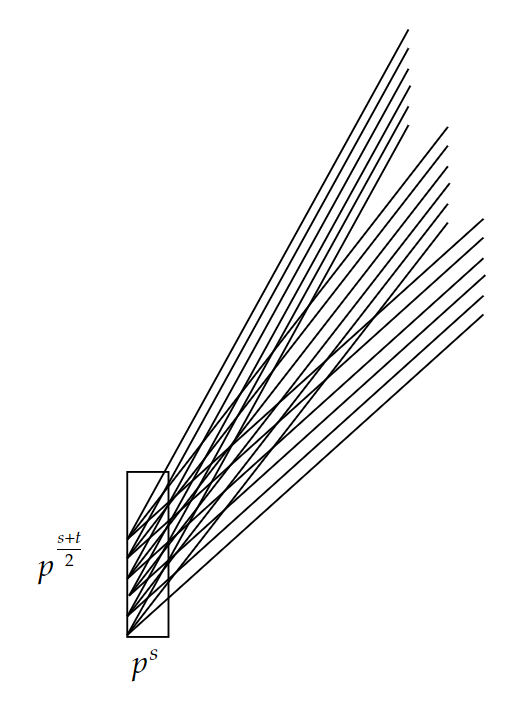
\includegraphics[width=5cm]{../assets/2476/F0.png}
\caption{}
\label{F0}
\end{minipage}
\end{figure}

\bigskip
% Original author source LF lines 745--766
\setcounter{theorem}{6}\setcounter{equation}{18}\setcounter{subsection}{1}
\subsection{Useful lemmas} We prove several useful lemmas, which will be used later in the proof. We suggest that the reader skip this part in the first reading. 




\begin{lemma} Suppose $G(k,\Fp^n)$ is the set of $k$-dimensional subspaces in $\Fp^n$, $A(k,\Fp^n)$ is the set of $k$-planes in $\Fp^n$. We have: 
\begin{enumerate}
    \item $\#G(k,\Fp^n)\sim p^{k(n-k)}$;
    \item $\# A(k,\Fp^n)\sim p^{(k+1)(n-k)}$;
    \item Fix integers $l,k$ with $l+k\ge n$. Let $W_0\in A(l,\Fp^n)$. Then $\#\{ V\in A(k,\Fp^n): V\cap W_0 \textup{~is~a~}(l+k-n)\textup{-plane} \}\gtrsim p^{(k+1)(n-k)}$.
\end{enumerate}
    
\end{lemma}
\begin{proof}
    (1) and (2) are fundamental.
    We prove (3). $V\cap W_0$ is a $(l+k-n)$-plane means $V$ intersects $W_0$ transversely. (3) agrees with intuition in $\R^n$, since generic $V\in A(k,\R^n)$ intersect $W_0$ transversely. Noting (2), we see that it suffices to prove 
    \begin{equation}\label{rplane}
        \#\{ V\in A(k,\Fp^n): V\cap W_0 \textup{~is~a~}r\textup{-plane} \}\lesssim p^{(k+1)(n-k)-1}, 
    \end{equation} 
    for $r>l+k-n$.
    The proof of \eqref{rplane} is as follows. Choose a $r$-plane $L$ in $W_0$. There are $\#G(r,\Fp^l)\sim p^{(r+1)(l-r)}$ choices for $L$. If $V\cap W_0=L$, then $V\supset L$. We have $\le \#\{V\in A(k,\Fp^n): V\supset L\}=\#G(k-r,\Fp^{n-r})\sim p^{(k-r)(n-k)}$ choices for $V$ such that $V\cap W_0=L$. The two estimates give \eqref{rplane}.
\end{proof}
% Original author source LF lines 956--1064
\setcounter{section}{2}\setcounter{equation}{23}
\section{Furstenberg set problem: upper bound}\label{sec3}

In this section, we prove Theorem \ref{upper bound}. In other words, we will construct a $(s,t;n,k)$-set $E=\bigcup_{V\in\cV}Y(V)$, such that
\[ \#E\lesssim_{s,t,n,k} p^{\bF(s,t;n,k)}.\]
  

\subsection{Two special cases} To familiarize ourselves with $\bF(s,t;n,k)$, we discuss two special cases: $s=k$; $k=1$.

When $s=k$, we can morally view $Y(V)$ as $V$. Therefore, a $(k,t;n,k)$-set is of the form
\[ E=\bigcup_{V\in\cV}V. \]
Estimating the size of $E$ is known as the problem of ``union of $k$ planes". It has been resolved in finite fields by R. Oberlin \cite{oberlin2016unions}. The Euclidean version was resolved by the author in \cite{gan2023hausdorff}.

When $k=1$, this is the Furstenberg set problem for lines. To construct a $(s,t;n,1)$-set 
\[ E=\bigcup_{L\in\cL}Y(L) \]
with size as small as possible, we hope that the lines in $\cL$ are compressed in a low-dimensional space. 
Write $t=2m+\beta$, where $0\le m\le n-2$ is an integer, and $\beta\in (0,2]$. Since $t\le 2(m+1)$, we can make $\cL$ contained in $\Fp^{m+2}$. Therefore, our goal becomes to construct a small $(s,t;m+2,1)$-set. The trick is to take the Cartesian product of a $(s,\beta;2,1)$-set with $\Fp^m$. Let $E'\subset \Fp^2$ be a $(s,\beta;2,1)$-set and let $E'$ have the form
\[ E'=\bigcup_{L'\in \cL'}Y(L'). \]
We will construct a $(s,t;m+2,1)$-set $E$ based on $E'$. Let $\pi_{\Fp^2}:\Fp^{m+2}\rightarrow \Fp^2$ be the projection onto the first two coordinates. Define $\cL$ to be the set of lines $L$ in $\Fp^{m+2}$ such that $\pi_{\Fp^2}(L)$ is a line in $\cL'$. Then, $\#\cL\sim \# G(1,\Fp^{m+1})\cdot \#\cL'\sim p^{2m+\beta}=p^t$. If $L\in \cL$, then $L'=\pi_{\Fp^2}(L)\in \cL'$. We define $Y(L):=L\cap \pi_{\Fp^2}^{-1}(Y(L'))$. We see that $\#Y(L)=\#Y(L')\sim p^s$, so 
\[ E=\bigcup_{L\in\cL}Y(L) \]
is a $(s,t;m+2,1)$-set.
Also, since $E\subset E'\times \Fp^m$, we have
\[ \#E\le\#E'\cdot p^m\lesssim p^{m+\min\{s+\beta,\frac32s+\frac12\beta,s+1\}}  \]
By checking Definition \ref{deffurindex}, one exactly sees that
    \[ m+\min\{s+\beta,\frac32s+\frac12\beta,s+1\}=\bF(s,t;m+2,1)=\bF(s,t;n,1). \]

\subsection{Proof of Theorem \ref{upper bound}}\hfill

For admissible $(s,t;n,k)$, we will construct a $(s,t;n,k)$-set 
\[ E=\bigcup_{V\in\cV}Y(V) \]
such that
\[ \#E\gtrsim p^{\bF(s,t;n,k)}. \]

\fbox{Case (a): \texorpdfstring{$s=0$}{}}

If $t\le k(n-k)$, we choose $\cV$ to be $p^t$ $k$-planes pass through the origin $\bzz^n$, and $Y(V)=\{\bzz^n\}$. Then $\#E\le 1=p^0$. Here, $\bzz^n$ means $(\underbrace{0,\dots,0}_{n \textup{~times~}})$.

If $t\ge k(n-k)$, we choose $p^{t-k(n-k)}$ points $X$ in $\Fp^{n-k}$. For each such point $x\in X$, we choose $\sim p^{k(n-k)}$ $k$-planes that pass through $x$, and require the $k$-planes to be transverse to $\Fp^{n-k}$. We obtain $\sim p^t$ $k$-planes which is $\cV$. If $V$ passes through $x\in X$, we set $Y(V)=\{x\}$. We see that $\#E=\#X\le p^{t-k(n-k)}$.

\bigskip

\fbox{Case (b): $s>0, t\in [0,(k-d-1)(n-k)]$}

We write $s=d+\si$, where $d\in \{0,\dots,k-1\}, \si\in(0,1]$.
The construction is similar to Case (a). We choose $\sim p^t$ many $k$-planes that contain $\Fp^{d+1}$. This is doable since 
\[ \#\{ V\in A(k,\Fp^n): V\supset L \}=\#G(k-d-1,\Fp^{n-d-1})\sim p^{(k-d-1)(n-k)}. \]
Let $\cV$ be these $k$-planes. Fix $Y\subset \Fp^{d+1}$ with $\#Y=p^s$. For each $V\in \cV$, let $Y(V)=Y$. We see that $\#E=\#Y=p^s$.





\bigskip

\fbox{Case (c): $s\in (0,k], t\in ((k-d-1)(n-k),(k+1)(n-k)]$}

We write 
\begin{equation}\label{stformula}
    \begin{cases}
        s=d+\si\\
        t=(k-d-1)(n-k)+(d+2)m+\tau,
    \end{cases}
\end{equation} 
    where $d\in\{0,\dots,k-1\}$, $\si\in (0,1]$,  $m\in\{0,\dots,n-k-1\}$, $\tau\in [0,2]$. We remark that here we allow $\tau=0$, although we assumed $\tau>$ in the canonical expression. Allowing $\tau=0$ will produce the example in Case (d).

We write $\Fp^n=\Fp^{n-k+d+1}\times \F_p^{k-d-1}$. Note that $\gtrsim 1$ fraction of $k$-planes intersect $\Fp^{n-k+d+1}$ at a $(d+1)$-plane. Heuristically speaking, to make $\#E$ as small as possible, we would like $E$ to be a subset of $\F_p^{n-k+d+1}\times \bzz^{k-d-1}$. For simplicity, we write $\F_p^{n-k+d+1}\times \bzz^{k-d-1}$ as $\Fp^{n-k+d+1}$, thinking of it as a subspace of $\Fp^n$. This will not cause any ambiguity.

Note that for each $W\in A(d+1,\F_p^{n-k+d+1})$, the cardinality of 
\[\{V\in A(k,\Fp^n): V\supset W,  V \textup{~is~transverse~to~} \F_p^{n-k+d+1} \}\] 
is $\sim \#G(k-d-1,\Fp^{n-k})\sim p^{(k-d-1)(n-k)}$. We just need to find $\cW\subset A(d+1,\F_p^{n-k+d+1})$ with $\#\cW\sim p^{t-(k-d-1)(n-k)}=p^{(d+2)m+\tau}$, and for each $W\in\cW$, to find $Y(W)\subset W$ with $\#Y(W)\sim p^{s}$, such that
\begin{equation}\label{constructW}
    \#\bigcup_{W\in\cW} Y(W)\lesssim p^{\bF(s,t;n,k)}.
\end{equation}

If this is done, then we let $\cV$ be those $k$-planes $V$ that contain some $W\in\cW$, and $Y(V)=Y(W)$ if $V\supset W$. We see that $\#\cV\sim \#\{W\}\cdot p^{(k-d-1)(n-k)}\sim p^t$, and hence $E=\bigcup_{V\in\cV} Y(V)$ is a $(s,t;n,k)$-set. Also, we have the upper bound
\[ \#E=\#\bigcup_{W\in\cW} Y(W)\lesssim p^{\bF(s,t;n,k)}. \]

It suffices to find a $(s,(d+2)m+\tau;n-k+d+1,d+1)$-set $E_1=\bigcup_{W\in\cW} Y(W)$ such that \eqref{constructW} holds. 
Note that $\#A(d+1,\Fp^{m+d+2})\sim p^{(d+2)(m+1)}$ and $(d+2)m+\tau\le (d+2)(m+1)$. We will construct the $(d+1)$-planes $\cW$ so that they lie in $\Fp^{m+d+2}$. 
It suffices to find a $(s,(d+2)m+\tau;m+d+2,d+1)$-set $E_1=\bigcup_{W\in\cW} Y(W)$ such that \eqref{constructW} holds.

We write $\Fp^{m+d+2}=\Fp^{d+2}\times\Fp^{m}=\Fp^2\times \Fp^d\times \Fp^m$. We first choose a $(\si,\tau;2,1)$-set $E_2=\bigcup_{L\in\cL}Y(L)$ in $\Fp^2$, such that
\[\#E_2\lesssim p^{\min\{\si+\tau,\frac32\si+\frac12\tau,\si+1\}}. \]
The existence of $E_2$ was shown in Proposition \ref{prop2d}.

Next, we define $\cU:=\{L\times \Fp^d: L\in\cL\}$ which is a subset of $A(d+1,\Fp^{d+2})$. And for each $U=L\times \Fp^d\in\cU$, define $Y(U)=Y(L)\times \Fp^d$. We see that $\#\cU= \#\cL\sim p^\tau$, $\#Y(U)=\#Y(L)\cdot p^d\sim p^{\si+d}=p^s$. We also see that $E_3:=\bigcup_{U\in \cU}Y(U)$ is contained in $E_2\times \Fp^d$, and hence \[\#E_3\lesssim p^{d+\min\{\si+\tau,\frac32\si+\frac12\tau,\si+1\}}.\]

Finally, we define $\cW$. For each $U\in \cU$, consider the $(m+d+1)$-plane $U\times \Fp^m$.
Let $\pi_U:U\times \Fp^m\rightarrow U$ be the projection (naturally defined). We let $\cW_U$ be the set of $(d+1)$-planes $W$ contained in $U\times \Fp^m$ such that $\pi_U(W)=U$. Note that $\gtrsim 1$ fraction of the $(d+1)$-planes in  $U\times \Fp^m$ lie in $\cW_U$, so $\#\cW_U\sim \#A(d+1,\Fp^{m+d+1})\sim p^{(d+2)m}$.

We define $\cW=\bigcup_{U\in \cU}\cW_U$ (actually this is a disjoint union). For $W\in \cW_U$, define $Y(W)=W\cap \pi_U^{-1}(Y(U))$. We see that $\#\cW\sim \#\cU\cdot p^{(d+2)m}\sim p^{(d+2)m+\tau}$, and $\#Y(W)=\#Y(U)\sim p^s$. Hence, $E_1=\bigcup_{W\in\cW}Y(W)$ is a $(s,(d+2)m+\tau;m+d+2,d+1)$-set. Since $E_1\subset E_3\times \Fp^m$, we have
\[ \#E_1\le \#E_3\cdot p^m\lesssim p^{d+m+\min\{\si+\tau,\frac32\si+\frac12\tau,\si+1\}}. \]
The construction is done.

\bigskip
\fbox{Case (d)}

We still use \eqref{stformula}, but the range of $\tau$ is $\tau\in(2,d+2]$. Note that the worst case is when $\tau=d+2$.
What we need to do is for
\begin{equation}
    \begin{cases}
        s=d+\si\\
        t=(k-d-1)(n-k)+(d+2)(m+1),
    \end{cases}
\end{equation} 
construct a $(s,t;n,k)$-set $E$ such that
\[ \#E\lesssim p^{s+m+1}. \]
The trick is to still use the construction in Case (c), with $\tau$ replaced by $0$ and $m$ replaced by $m+1$. Therefore, we can construct a $(s,t;n,k)$-set $E$ such that
\[\#E\lesssim p^{d+m+1+\min\{\si+0,\frac32\si+\frac120,\si+1\}=p^{d+m+1+\si}=p^{s+m+1}}. \]
\
\clearpage
\section*{Editable original figure-label transcription}
\noindent The unchanged original Figure 1 above contains two printed mathematical labels. Their exact editable transcriptions and positions follow; no inferred diagram label or new argument is added.
\begin{itemize}
\item $p^{\frac{s+t}{2}}$: to the left of the rectangle, vertical extent label.
\item $p^s$: below the rectangle, horizontal extent label.
\end{itemize}
\begin{thebibliography}{99}
\bibitem[7]{gan2023hausdorff}
S.~Gan.
\newblock Hausdorff dimension of unions of $k$-planes.
\newblock {\em arXiv preprint arXiv:2305.14544}, 2023.

\bibitem[15]{oberlin2016unions}
R.~Oberlin.
\newblock Unions of lines in ${F}^n$.
\newblock {\em Mathematika}, 62(3):738--752, 2016.

\bibitem[17]{orponen2023projections}
T.~Orponen and P.~Shmerkin.
\newblock Projections, {F}urstenberg sets, and the $ {ABC} $ sum-product problem.
\newblock {\em arXiv preprint arXiv:2301.10199}, 2023.

\bibitem[19]{ren2023furstenberg}
K.~Ren and H.~Wang.
\newblock {F}urstenberg sets estimate in the plane.
\newblock {\em arXiv preprint arXiv:2308.08819}, 2023.

\bibitem[20]{wolff1999recent}
T.~Wolff.
\newblock Recent work connected with the {K}akeya problem.
\newblock {\em Prospects in mathematics (Princeton, NJ, 1996)}, 2(129-162):4, 1999.


\end{thebibliography}\end{document}
